\documentclass[a5paper]{article}
\usepackage{graphicx}
\usepackage{hyperref}
\usepackage[final]{pdfpages}
\usepackage[parfill]{parskip}% don't indent new sections
\usepackage[utf8]{inputenc}
\usepackage{listings}
\usepackage{color}
\usepackage[a4paper]{geometry}
\pagestyle{empty}

\definecolor{dkgreen}{rgb}{0,0.6,0}
\definecolor{gray}{rgb}{0.5,0.5,0.5}
\definecolor{mauve}{rgb}{0.58,0,0.82}

\lstset{frame=tb,
    language=Java,
    aboveskip=3mm,
    belowskip=3mm,
    showstringspaces=false,
    columns=flexible,
    basicstyle={\small\ttfamily},
    numbers=none,
    numberstyle=\tiny\color{gray},
    keywordstyle=\color{blue},
    commentstyle=\color{dkgreen},
    stringstyle=\color{mauve},
    breaklines=true,
    breakatwhitespace=true,
    tabsize=3
}

\title{Practical Concurrent and Parallel Programming}
\author{Emil Lynegaard}

\begin{document}

\includepdf[pages=1]{res/front_page.pdf}
\maketitle
\textit{I hereby declare that I have answered thede exam questions myself without any outside help.}\\

Through all tests, the same machine will be used. Below are the results of \texttt{SystemInfo}:


\begin{table}[!ht]
\begin{center}
\begin{tabular}{ l l }
OS & Linux; 4.13.12-1-ARCH; amd64\\
JVM & Oracle Corporation; 1.8.0\_144\\
CPU & null; 8 "cores"\\
Date & 2017-12-11T09:20:13+0100
\end{tabular}
\end{center}
\caption{System Info}
\label{sysinfo}
\end{table}

\section{Question 1}
\subsection{}
Seeing as we are interested in seeing how well each implementation performs on random input of different sizes, we use Mark9 for the benchmarking, as it calculates the per element mean time and standard deviation.

\begin{figure}[!ht]
    \centering
    \noindent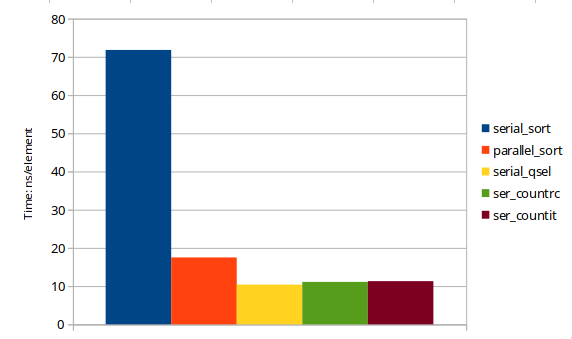
\includegraphics[scale=0.5]{res/graph_q1.png}
    \caption{Plot of running times of given implementations. Tested with size = 10000000.}
    \label{fig:graphq1}
\end{figure}

From graph \ref{fig:graphq1} we see that, perhaps unsurprisingly, the serial quickselect and quickcount implementations beat out serial sort entirely.
We do however see parallel sort get rather close to the expected linear running time implementations, due to the test machine having a quad-core CPU,
allowing an approximate 4 time speedup from the serial implementation. Between the expected linear running time algorithms, it seems serial quickselect 
beat out its quickcount counterparts, however the difference is so small that we have yet to find a definitive winner.

\subsection{}


\section{Question 2}
\subsection{}
\begin{lstlisting}
      (int) Arrays.stream(inp).skip(1).filter(i -> i < p).count();
\end{lstlisting}
Where \texttt{inp} is our input array, and \texttt{p} is our current partition candidate.
Skip the first element as this is the index of the partition element with which we do not wish to compare.

\subsection{}
\begin{lstlisting}
          Arrays.stream(inp).skip(1).filter(i -> i < p).toArray();
          Arrays.stream(inp).skip(1).filter(i -> i >= p).toArray();
\end{lstlisting}

\subsection{}
\begin{lstlisting}
public static int quickCountStream(int[] inp) {
    int partition=-1, count=0, n=inp.length;
    int target = n/2;
    do {
        partition=inp[0];
        final int p = partition;
        n=inp.length;
        count = (int) Arrays.stream(inp).skip(1).filter(i -> i < p).count();
        if (count == target) break;
        if (count > target){
            inp = Arrays.stream(inp).skip(1).parallel.()filter(i -> i < p).toArray();
        }else{
            inp = Arrays.stream(inp).skip(1).parallel().filter(i -> i >= p).toArray();
            target=target-count-1;
        }
    } while( true );
    return partition; // we are on target
}
\end{lstlisting}

Combining the two we get above implementation, which yields correct results.

\subsection{}
\begin{lstlisting}
    Arrays.stream(inp).parallel().skip(1).filter(i -> i < p).count();
    Arrays.stream(inp).parallel().skip(1).filter(i -> i < p).toArray();
    Arrays.stream(inp).parallel().skip(1).filter(i -> i >= p).toArray();
\end{lstlisting}
Here we simply throw \texttt{.parallel()} onto the pipelines from before.

\subsection{}
\end{document}
